\documentclass{article}

\usepackage[T1]{fontenc}

\usepackage{fancyhdr}
\usepackage{extramarks}
\usepackage{amsmath}
\usepackage{amsthm}
\usepackage{amsfonts}
\usepackage{tikz}
\usepackage{algorithm}
\usepackage{algpseudocode}
\usepackage{enumitem}

\usepackage[mono=false]{libertine}


\usetikzlibrary{automata,positioning}

%
% Basic Document Settings
%

\topmargin=-0.45in
\evensidemargin=0in
\oddsidemargin=0in
\textwidth=6.5in
\textheight=9.0in
\headsep=0.25in

\linespread{1.1}

\pagestyle{fancy}
\lhead{\hmwkAuthorName}
\chead{\hmwkClass: \hmwkTitle}
\rhead{\firstxmark}
\lfoot{\lastxmark}
\cfoot{\thepage}

\renewcommand\headrulewidth{0.4pt}
\renewcommand\footrulewidth{0.4pt}

\setlength\parindent{0pt}

%
% Create Problem Sections
%

\newcommand{\enterProblemHeader}[1]{
    \nobreak\extramarks{}{Problem \arabic{#1} continued on next page\ldots}\nobreak{}
    \nobreak\extramarks{Problem \arabic{#1} (continued)}{Problem \arabic{#1} continued on next page\ldots}\nobreak{}
}

\newcommand{\exitProblemHeader}[1]{
    \nobreak\extramarks{Problem \arabic{#1} (continued)}{Problem \arabic{#1} continued on next page\ldots}\nobreak{}
    \stepcounter{#1}
    \nobreak\extramarks{Problem \arabic{#1}}{}\nobreak{}
}

\setcounter{secnumdepth}{0}
\newcounter{partCounter}
\newcounter{homeworkProblemCounter}
\setcounter{homeworkProblemCounter}{1}
\nobreak\extramarks{Problem \arabic{homeworkProblemCounter}}{}\nobreak{}

%
% Homework Problem Environment
%
% This environment takes an optional argument. When given, it will adjust the
% problem counter. This is useful for when the problems given for your
% assignment aren't sequential. See the last 3 problems of this template for an
% example.
%
\newenvironment{homeworkProblem}[1][-1]{
    \ifnum#1>0
        \setcounter{homeworkProblemCounter}{#1}
    \fi
    \section{Problem \arabic{homeworkProblemCounter}}
    \setcounter{partCounter}{1}
    \enterProblemHeader{homeworkProblemCounter}
}{
    \exitProblemHeader{homeworkProblemCounter}
}

%
% Homework Details
%   - Title
%   - Due date
%   - Class
%   - Section/Time
%   - Instructor
%   - Author
%

\newcommand{\hmwkTitle}{Homework\ \#4}
\newcommand{\hmwkDueDate}{March 27, 2018}
\newcommand{\hmwkClass}{Design and Analysis of Algorithms}
\newcommand{\hmwkClassInstructor}{Professor Kasturi Varadarajan}
\newcommand{\hmwkAuthorName}{\textbf{Alic Szecsei}}

%
% Title Page
%

\title{
    \vspace{2in}
    \textmd{\textbf{\hmwkClass:\ \hmwkTitle}}\\
    \normalsize\vspace{0.1in}\small{Due\ in\ class\ on\ \hmwkDueDate}\\
    \vspace{0.1in}\large{\textit{\hmwkClassInstructor}}
    \vspace{3in}
}

\author{\hmwkAuthorName}
\date{}

\renewcommand{\part}[1]{\textbf{\large Part \Alph{partCounter}}\stepcounter{partCounter}\\}

%
% Various Helper Commands
%

% Useful for algorithms
\newcommand{\alg}[1]{\textsc{\bfseries \footnotesize #1}}

% For derivatives
\newcommand{\deriv}[1]{\frac{\mathrm{d}}{\mathrm{d}x} (#1)}

% For partial derivatives
\newcommand{\pderiv}[2]{\frac{\partial}{\partial #1} (#2)}

% Integral dx
\newcommand{\dx}{\mathrm{d}x}

% Alias for the Solution section header
\newcommand{\solution}{\textbf{\large Solution}}

% Probability commands: Expectation, Variance, Covariance, Bias
\newcommand{\E}{\mathrm{E}}
\newcommand{\Var}{\mathrm{Var}}
\newcommand{\Cov}{\mathrm{Cov}}
\newcommand{\Bias}{\mathrm{Bias}}

% Set from 1 to N
\newcommand{\XYZ}[1]{\left\{1,\ldots,{#1}\right\}}
\newcommand{\Break}{\textbf{break} }

\begin{document}

\maketitle

\pagebreak

\begin{homeworkProblem}

Consider the following randomized algorithm for generating biased random bits. The subroutine \alg{FairCoin} returns either 0 or 1 with equal probability; the random bits returned by \alg{FairCoin} are mutually independent.

\begin{algorithm}
	\begin{algorithmic}[1]
		\Function{OneInThree}{}
			\If{\Call{FairCoin}{} $= 0$}
				\State{\Return{0}}
			\Else
				\State{\Return{$1 - $\Call{OneInThree}{}}}
			\EndIf
		\EndFunction
	\end{algorithmic}
\end{algorithm}

\begin{enumerate}[label=(\alph*)]
	\item Prove that \alg{OneInThree} returns 1 with probability $\frac{1}{3}$.
	\item What is the \emph{exact} expected number of times that this algorithm calls \alg{FairCoin}?
	\item Now suppose you are \emph{given} a subroutine \alg{OneInThree} that generates a random bit that is equal to 1 with probability $\frac{1}{3}$. Describe a \alg{FairCoin} algorithm that returns either 0 or 1 with equal probability, using \alg{OneInThree} as your only source of randomness.
	\item What is the \emph{exact} expected number of times that your \alg{FairCoin} algorithm calls \alg{OneInThree}?
\end{enumerate}

\solution\\

\part

In order for \alg{OneInThree} to return 1, \alg{FairCoin} must return an odd number of 1s before returning a 0. We can begin to enumerate cases: first, that \alg{FairCoin} returns a 1 and then a 0 is $\frac{1}{2} \cdot \frac{1}{2} = \frac{1}{4}$. The probability that \alg{FairCoin} returns 3 1s and then a 0 is $\frac{1}{2} \cdot \frac{1}{2} \cdot \frac{1}{2} \cdot \frac{1}{2} = \frac{1}{16}$. The probability that \alg{FairCoin} returns 5 1s and then a 0 is $\frac{1}{2} \cdot \frac{1}{2} \cdot \frac{1}{2} \cdot \frac{1}{2} \cdot \frac{1}{2} \cdot \frac{1}{2} = \frac{1}{64}$, and so on. Our summation of all cases is then:
\begin{equation}
\frac{1}{4} + \frac{1}{16} + \frac{1}{64} + \ldots + \frac{1}{2^{2n}} = \sum_{k = 1}^{\infty} \frac{1}{2^{2k}}
\end{equation}

This is a geometric series with common ratio $r = \frac{1}{4}$; we can then use the formula $S = \frac{a_1}{1 - r}$ to determine the summation. Using this, we can see that $S = \frac{\frac{1}{4}}{1 - \frac{1}{4}} = \frac{\frac{1}{4}}{\frac{3}{4}} = \frac{1}{3}$. Therefore, \alg{OneInThree} has a $\frac{1}{3}$ probability of returning 1.\\

\part

Since \alg{OneInThree} might never terminate, our expected value of $T(n)$ is:
\begin{equation}
	E[T(n)] = \sum_{k = 1}^\infty k \cdot \text{Pr}[T(n) = k]
\end{equation}

In order for \alg{OneInThree} to terminate with exactly $k$ calls to \alg{FairCoin}, there must have been exactly $k-1$ times that \alg{FairCoin} returned 1 (and \alg{OneInThree} continued recursing), and 1 time it returned 0 (and \alg{OneInThree} stopped recursing). Thus, the combined probability for \alg{OneInThree} to terminate with exactly $k$ calls to \alg{FairCoin} is $\frac{1}{2^k}$. Plugging this back into our equation for $E[T(n)]$:

\begin{equation}
	\begin{split}
		E[T(n)] &= \sum_{k = 1}^\infty k \cdot \text{Pr}[T(n) = k]\\
		&= \sum_{k = 1}^\infty k \cdot \frac{1}{2^k}\\
		&= 2
	\end{split}
\end{equation}

\part

\begin{algorithm}
	\begin{algorithmic}[1]
		\Function{FairCoin}{}
			\State{$c_1 \gets \Call{OneInThree}{}$}
			\State{$c_2 \gets \Call{OneInThree}{}$}
			\If{$c_1 = 1$ and $c_2 = 1$}
				\State{\Return{\Call{FairCoin}{}}}
			\Else
				\If{$c_1 = 1$ or $c_2 = 1$}
					\State{\Return{$1$}}
				\Else
					\State{\Return{$0$}}
				\EndIf
			\EndIf
		\EndFunction
	\end{algorithmic}
\end{algorithm}

The idea for this algorithm is that we break the probability space into 3 partitions: first, the probability that both calls to \alg{OneInThree} return $1$ is $\frac{1}{9}$. The remaining probability is $\frac{8}{9}$; we further divide this into two partitions. The probability that both calls to \alg{OneInThree} returned $0$ is $\frac{4}{9}$; thus, the remaining probability (that only one call to \alg{OneInThree} returned $1$) is $\frac{4}{9}$.\\

Now, the probability that any call to \alg{FairCoin} which actually \emph{returns} will return 0 is clearly $\frac{1}{2}$; the same probability applies to any returning call to \alg{FairCoin} returning 1. Thus, \alg{FairCoin} has an equal probability of returning either 0 or 1.\\

\part

Since \alg{FairCoin} might never terminate, our expected value of $T(n)$ is:
\begin{equation}
	E[T(n)] = \sum_{k = 1}^\infty k \cdot \text{Pr}[T(n) = k]
\end{equation}

In order for \alg{FairCoin} to terminate with exactly $2k$ calls to \alg{OneInThree}, there must have been exactly $k-1$ times that both calls of \alg{OneInThree} returned 1 (and \alg{FairCoin} continued recursing), and 1 time at least one call returned 0 (and \alg{FairCoin} stopped recursing). Thus, the combined probability for \alg{FairCoin} to terminate with exactly $2k$ calls to \alg{FairCoin} is $\frac{1}{9^{k-1}} \cdot \frac{8}{9} = \frac{8}{9^k}$. Plugging this back into our equation for $E[T(n)]$:

\begin{equation}
	\begin{split}
		E[T(n)] &= \sum_{k = 1}^\infty 2k \cdot \text{Pr}[T(n) = k]\\
		&= \sum_{k = 1}^\infty 2k \cdot \frac{8}{9^k}\\
		&= \frac{9}{4}
	\end{split}
\end{equation}

\end{homeworkProblem}

\pagebreak

\begin{homeworkProblem}

Consider the following algorithm for finding the smallest element in an unsorted array:

\begin{algorithm}
	\begin{algorithmic}[1]
		\Function{RandomMin}{$A[1..n]$}
			\State{$min \gets \infty$}
			\For{$i \gets 1$ to $n$ in random order}
				\If{$A[i] < min$}
					\State{$min \gets A[i]$}\Comment{$(\star)$}
				\EndIf
			\EndFor
			\State{\Return{$min$}}
		\EndFunction
	\end{algorithmic}
\end{algorithm}

\begin{enumerate}[label=(\alph*)]
	\item In the worst case, how many times does \alg{RandomMin} execute line $(\star)$?
	\item What is the probability that line $(\star)$ is executed during the $i$th iteration of the for loop?
	\item What is the \emph{exact} expected number of executions of line $(\star)$?
\end{enumerate}

\solution\\

\part

In the worst case, \alg{RandomMin} retrieves the elements in descending order, so it must re-assign $min$ (in line $(\star)$) a total of $n$ times.\\

\part

If line $(\star)$ is executed during the $i$th iteration of the for loop, this means that the randomly selected element is smaller than the previous $i-1$ randomly selected elements. Essentially, we have a set of $i$ elements, and we want to know the probability that a specific element (the most recently added element) is the smallest element in that set. We have a single minimal element, and a $\frac{1}{i}$ chance of choosing that minimal element; therefore, the probability that the most recently added element is the minimal element of the set is $\frac{1}{i}$. We can thus conclude that the probability that line $(\star)$ is executed during the $i$th iteration of the for loop is also $\frac{1}{i}$.\\

\part

We know that line $(\star)$ has a $\frac{1}{i}$ probability of being executed during the $i$th iteration of the for loop, so the expected value at each iteration of the for loop is:

\begin{equation}
	E[T(n)]_{\text{iter}} = 0 \cdot \frac{i-1}{i} + 1 \cdot \frac{1}{i} = \frac{1}{i}
\end{equation}

We can sum all of these expected values together to determine the expected number of executions of line $(\star)$ during the entire algorithm:

\begin{equation}
	E[T(n)] = \sum_{k = 1}^{n} \frac{1}{k} = H_n
\end{equation}

\end{homeworkProblem}

\pagebreak

\begin{homeworkProblem}

Suppose we have a circular linked list of numbers, implemented as a pair of arrays, one storing the actual numbers and the other storing successor pointers. Specifically, let $X[1..n]$ be an array of $n$ distinct real numbers, and let $N[1..n]$ be an array of indices with the following property: If $X[i]$ is the largest element of $X$, then $X[N[i]]$ is the smallest element of $X$; otherwise, $X[N[i]]$ is the smallest among the set of elements in $X$ larger than $X[i]$. For example:

\begin{table}[h]
	\centering
		\begin{tabular}{r | *{9}{c} }
			$i$    &  1 &  2 &  3 &  4 &  5 &  6 &  7 &  8 &  9 \\
			\hline
			$X[i]$ & 83 & 54 & 16 & 31 & 45 & 99 & 78 & 62 & 27 \\
			\hline
			$N[i]$ &  6 &  8 &  9 &  5 &  2 &  3 &  1 &  7 &  4
		\end{tabular}
\end{table}

Describe and analyze a randomized algorithm that determines whether a given number $x$ appears in the array $X$ in $O(\sqrt{n})$ expected time. \emph{\textbf{Your algorithm may not modify the arrays $X$ and $N$.}}\\

\solution\\

\begin{algorithm}
	\begin{algorithmic}[1]
		\Function{RandomContains}{$X[1..n], N[1..n], x$}
			\State{$T \gets$ an array of $\sqrt{n}$ random numbers between 1 and $n$}
			\State{$hasLowerBound \gets False$} \Comment{We need to be able to handle the case where we do not select any elements less than $x$}
			\For{$i \gets 1, \sqrt{n}$}
				\If{$X[T[i]] < x$}
					\State{$hasLowerBound \gets True$}
					\Break
				\EndIf
			\EndFor
			\If{$hasLowerBound$}
				\State{$minDist \gets \infty$}
				\For{$i \gets 1, \sqrt{n}$}
					\If{$X[T[i]] < x$ and $x - X[T[i]] < minDist$}
						\State{$minDist \gets x - X[T[i]]$}
						\State{$l \gets T[i]$}
					\EndIf
				\EndFor
			\Else
				\State{$l \gets T[1]$}
				\For{$i \gets 2, \sqrt{n}$}
					\If{$X[T[i]] > X[l]$}
						\State{$l \gets T[i]$}
					\EndIf
				\EndFor
			\EndIf \Comment{We now have the ``closest'' element before $x$ (if it exists) on our linked list}
			\While{$True$}
				\If{$X[l] = x$}
					\State{\Return{$True$}}
				\Else
					\State{$prev \gets X[l]$}
					\State{$l \gets N[l]$}
					\If{$X[l] < prev$}
						\If{$hasLowerBound$}
							\State{\Return{$False$}} \Comment{We wrapped around before we found $x$}
						\Else
							\State{$hasLowerBound \gets True$} \Comment{We wrapped around, so we \emph{should} have a lower bound}
						\EndIf
					\EndIf
					\If{$X[l] > x$ and $hasLowerBound$}
						\State{\Return{$False$}} \Comment{We had a lower bound, but now we've passed where $x$ should have been}
					\EndIf
				\EndIf
			\EndWhile
		\EndFunction
	\end{algorithmic}
\end{algorithm}

Our algorithm selects $\sqrt{n}$ random pivots in the linked list, and searches them to find the greatest lower bound on our target value. If our target value is less than all of the pivots, it selects the largest pivot. We then walk through the linked list until we either find our target or exceed its value (with suitable edge cases handled if we need to wrap around).\\

First, we would like to show that the expected size $S$ of any of the $\sqrt{n}$ partitions our algorithm generates is, itself, $\sqrt{n}$. As an example, we will have 3 partitions of an array of length 9. We randomly select an element of the array $r$ and two pivots, $p_1$ and $p_2$; without loss of generality, assume $p_1 < p_2$. The probability that $r$ is between the two pivots is $\frac{1}{3}$, as the other two equiprobable alternatives are that $r < p_1$ and $r > p_2$. The probability that any value is in one of the partitions is $\frac{S}{L}$, where $L$ is the length of the array and $S$ is the partition size; thus, the expected length of each partition must be $\frac{1}{3} = \frac{S}{L} \Rightarrow \frac{1}{3} = \frac{S}{9} \Rightarrow S = 3$.\\

We can generalize this for any array length $L$ and number of partitions $P$; the expected partition size must be $\frac{L}{P}$. Since we have $\sqrt{n}$ partitions and an array of size $n$, our expected partition size is $\frac{n}{\sqrt{n}} = \sqrt{n}$.\\

Our algorithm uses $O(\sqrt{n})$ runtime to generate our pivot list and determine which partition contains $x$; it then linearly traverses the relevant partition. Since our expected partition size is \emph{also} $\sqrt{n}$, we can determine our final expected runtime to be $O(\sqrt{n})$.

\end{homeworkProblem}

\pagebreak

\begin{homeworkProblem}

A \emph{majority tree} is a complete ternary tree with depth $n$, where every leaf is labeled either 0 or 1. The \emph{value} of a leaf is its label; the \emph{value} of any internal node is the majority of the values of its three children. Consider the problem of computing the value of the root of a majority tree, given the sequence of $3^n$ leaf labels as input. For example, if $n = 2$ and the leaves are labeled 1, 0, 0, 0, 1, 0, 1, 1, 1, the root has value 0.

\begin{figure}[h]
	\centering
		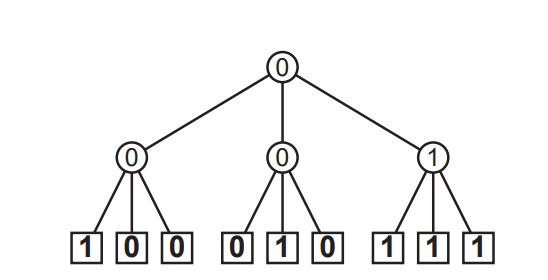
\includegraphics{images/majoritytree.png}
	\caption{A majority tree with depth $n = 2$.}
	\label{fig:majoritytree}
\end{figure}

\begin{enumerate}[label=(\alph*)]
	\item Prove that \emph{any} deterministic algorithm that computes the value of the root of a majority tree \emph{must} examine every leaf. \emph{[Hint: Consider the special case $n = 1$. Recurse.]}
	\item Describe and analyze a randomized algorithm that computes the value of the root in worst-case expected time $O(c^n)$ for some constant $c < 3$. \emph{[Hint: Consider the special case $n = 1$. Recurse.}
\end{enumerate}

\solution\\

\part

In order to determine the value of a node, a deterministic algorithm can use 1, 2, or 3 of its children's values. If an algorithm uses only one child, it has the obvious potential to be wrong (for example, one in which an algorithm only examines a child of value \textbf{1}, while the other two children both have values of \textbf{0}). If an algorithm only examines 2 of its children's values, it can encounter a tie (in which the algorithm examines children of values \textbf{0} and \textbf{1}). It cannot determine which of these values to correctly return \emph{unless} the algorithm also references the third child (as the third child may be either \textbf{0} or \textbf{1}, acting as a tie-breaker). Therefore, for any non-leaf node, the algorithm must examine all 3 of the node's children. The algorithm must be called on every child of the root, and every grandchild, and so on. Since the root has all leaf nodes as its descendents, the algorithm will examine every descendent of the root, which includes all leaf nodes.\\

\part

\begin{algorithm}
	\begin{algorithmic}[1]
		\Function{Majority}{$N[1..n]$}
			\If{$n = 1$}
				\State{\Return{$N[1]$}}
			\Else
				\State{$p_1 \gets N[1..\frac{n}{3}]$}
				\State{$p_2 \gets N[\frac{n}{3}+1..\frac{2n}{3}]$}
				\State{$p_3 \gets N[\frac{2n}{3}+1..n]$}
				\State{$children \gets$ a shuffled list of $p_1$, $p_2$, and $p_3$}
				\State{$a \gets \Call{Majority}{children[0]}$}
				\State{$b \gets \Call{Majority}{children[1]}$}
				\If{$a = b$}
					\State{\Return{$a$}}
				\Else
					\State{\Return{\Call{Majority}{$children[2]$}}}
				\EndIf
			\EndIf
		\EndFunction
	\end{algorithmic}
\end{algorithm}

The base case of our algorithm is straightforward; if a node is a leaf (represented by a list containing only 1 element), its value can simply be returned.\\

The recursive case is somewhat more interesting; we retrieve two random children (sub-lists) of the node and examine their values. If they are the same, we can immediately return this value; no matter what the third child's value is, the majority is already known. However, if the values are \emph{not} the same, one must be a 0 and one must be a 1; the third child acts as a tiebreaker, and we can simply return its value.\\

In order to construct an expected runtime, we will assume that the worst-case problem is given; namely, that each possible decision contains a mixed distribution of \textbf{1}s and \textbf{0}s. Then, to determine expected runtime, we want to examine the expected number of recursive calls to \alg{Majority}. There's a $\frac{2}{3}$ chance of selecting one of the duplicate values for the first selection. After this, there is a $\frac{1}{2}$ chance of selecting the other duplicate value, for a total probability of $\frac{2}{6} = \frac{1}{3}$. In this case, we would perform 2 recursive calls. Conversely, there must be a $\frac{2}{3}$ probability that the first two calls to \alg{Majority} returned differing values; in this case, we would perform 3 recursive calls. Therefore, the expected number of recursive calls is $2 \cdot \frac{1}{3} + 3 \cdot \frac{2}{3} = \frac{8}{3}$.\\

We can use this to determine our runtime; namely, $T(n) = \frac{8}{3}T(n-1)$, as we run an expected $\frac{8}{3}$ recursions, and each child has depth of $n-1$. Using annihilators,

\begin{equation}
	\begin{split}
		T(n)   &= \frac{8}{3}T(n-1)   \\
		T(n+1) &= \frac{8}{3}T(n)     \\
		T(n+1) - \frac{8}{3}T(n) &= 0 \\
		\left(\textbf{E}-\frac{8}{3}\right)T(n) &= 0
	\end{split}
\end{equation}

Our annihilator is thus $(\textbf{E} - \frac{8}{3})$. This gives us the generic solution $T(n) = \alpha \frac{8}{3}^n$ for some unknown constant $\alpha$; therefore, this algorithm runs in $O(\frac{8}{3}^n)$ time.

\end{homeworkProblem}

\pagebreak

\begin{homeworkProblem}

Suppose you are given a graph $G$ with weighted edges, and your goal is to find a cut whose total weight (not just number of edges) is smallest.

\begin{enumerate}[label=(\alph*)]
	\item Describe an algorithm to select a random edge of $G$, where the probability of choosing edge $e$ is proportional to the weight of $e$.
	\item Prove that if you use the algorithm from part (a), instead of choosing edges uniformly at random, the probability that \alg{GuessMinCut} returns a minimum-weight is still $\Omega(1/n^2)$.
	\item What is the running time of your modified \alg{GuessMinCut} algorithm?
\end{enumerate}

\solution\\

\part

\begin{algorithm}
	\begin{algorithmic}[1]
		\Function{SelectEdge}{$G$}
			\State{$t \gets 0$}
			\ForAll{$e$ in $G.edges$}
				\State{$t \gets t + e.weight$} \Comment{Get total edge weights}
			\EndFor
			\State{$r \gets$ a random number between 0 and $t$}
			\State{$i \gets 0$} \Comment{$i$ accumulates edge weights until we pass our random number}
			\ForAll{$e$ in $G.edges$}
				\State{$i \gets i + e.weight$}
				\If{$i > r$}
					\State{\Return{$e$}}
				\EndIf
			\EndFor
		\EndFunction
	\end{algorithmic}
\end{algorithm}

\part

Assume without loss of generality that we are given a graph $G$ with $m$ edges, which has a unique min cut consisting of $k$ edges with weights $w_1, w_2, ..., w_k$. Let the weight of the min cut be $W_C$, and the weight of the graph be $\sum_{e \in E} w_e = W_G$.\\

We can define the probability that we choose an edge in the min cut as $\frac{W_C}{W_G}$. Since $W_C$ is weight of the min cut, we know that every possible vertex-isolating cut of $G$ must have a weight of at least $W_C$; that is, for all vertices $v$, the sum of the weights of all edges connected to $v$ must be greater than $W_C$.\\

For each vertex, we can obtain a vertex-isolating cut; which transforms our inequality into:

\begin{equation}
	\begin{split}
		\sum_{v \in V} \sum_{e = (v, v')} w_e &\geq \sum_{v \in V} W_C\\
		\sum_{v \in V} \sum_{e = (v, v')} w_e &\geq n \cdot W_C
	\end{split}
\end{equation}

The handshake lemma says that the sum of the degrees of all vertices is equal to $2m$, so our inequality can further be transformed into $2 \sum_{e \in E} w_e = 2 \cdot W_G \geq n \cdot W_C$. Simple algebra suffices to transform this into:

\begin{equation}
	\frac{W_C}{W_G} \leq \frac{2}{n}
\end{equation}

The event that we arrived at an optimal cut means that none of the edges within the cut was selected by our algorithm; the probability that no edge in the min cut was selected during an iteration is $1 - \frac{W_C}{W_G} \geq 1 - \frac{2}{n}$.\\

This matches the probability for the unmodified \alg{GuessMinCut} algorithm, so by the same logic as is used to determine that probability of success, the probability of success of our modified \alg{GuessMinCut} algorithm will \emph{also} be $\Omega(1/n^2)$.\\

\part

In order to determine the runtime of the modified \alg{GuessMinCut} algorithm, we need to first determine the runtime of our \alg{SelectEdge} algorithm. As this simply iterates twice over the number of edges in the graph, it has a $O(n^2)$ runtime complexity, since there are at most $\frac{n(n-1)}{2}$ edges in a graph.\\

The \alg{GuessMinCut} algorithm requires that we iterate over each vertex in $G$, picking random edges and collapsing them. Picking a random edge, as we just determined, requires $O(n^2)$ time, while collapsing an edge only requires $O(n)$ time. Therefore, the costly operation is picking a random edge, which must happen once for each vertex; the total runtime of the modified \alg{GuessMinCut} algorithm is thus $O(n^3)$.

\end{homeworkProblem}

\end{document}